

\tikzset{every picture/.style={line width=0.75pt}} %set default line width to 0.75pt        

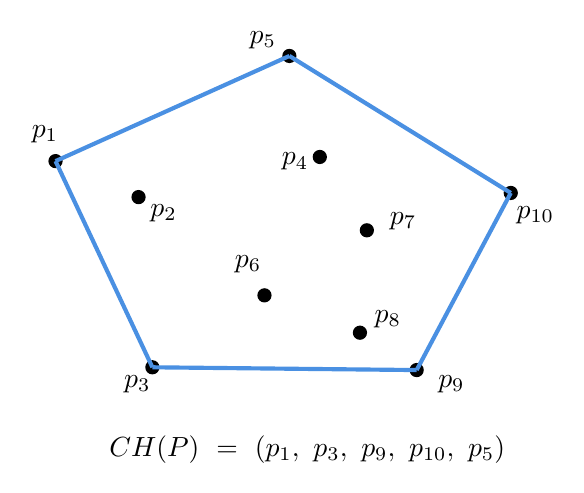
\begin{tikzpicture}[x=0.5pt,y=0.5pt,yscale=-1,xscale=1]
%uncomment if require: \path (0,420); %set diagram left start at 0, and has height of 420

%Flowchart: Connector [id:dp05090347480351787] 
\draw  [fill={rgb, 255:red, 0; green, 0; blue, 0 }  ,fill opacity=1 ] (57,162) .. controls (57,159.58) and (58.96,157.62) .. (61.38,157.62) .. controls (63.79,157.62) and (65.75,159.58) .. (65.75,162) .. controls (65.75,164.42) and (63.79,166.38) .. (61.38,166.38) .. controls (58.96,166.38) and (57,164.42) .. (57,162) -- cycle ;
%Flowchart: Connector [id:dp3291568735294871] 
\draw  [fill={rgb, 255:red, 0; green, 0; blue, 0 }  ,fill opacity=1 ] (226,86) .. controls (226,83.58) and (227.96,81.62) .. (230.38,81.62) .. controls (232.79,81.62) and (234.75,83.58) .. (234.75,86) .. controls (234.75,88.42) and (232.79,90.38) .. (230.38,90.38) .. controls (227.96,90.38) and (226,88.42) .. (226,86) -- cycle ;
%Flowchart: Connector [id:dp6621594719883535] 
\draw  [fill={rgb, 255:red, 0; green, 0; blue, 0 }  ,fill opacity=1 ] (318,313) .. controls (318,310.58) and (319.96,308.62) .. (322.38,308.62) .. controls (324.79,308.62) and (326.75,310.58) .. (326.75,313) .. controls (326.75,315.42) and (324.79,317.38) .. (322.38,317.38) .. controls (319.96,317.38) and (318,315.42) .. (318,313) -- cycle ;
%Flowchart: Connector [id:dp25920829224973985] 
\draw  [fill={rgb, 255:red, 0; green, 0; blue, 0 }  ,fill opacity=1 ] (127,311) .. controls (127,308.58) and (128.96,306.62) .. (131.38,306.62) .. controls (133.79,306.62) and (135.75,308.58) .. (135.75,311) .. controls (135.75,313.42) and (133.79,315.38) .. (131.38,315.38) .. controls (128.96,315.38) and (127,313.42) .. (127,311) -- cycle ;
%Flowchart: Connector [id:dp02220382507011076] 
\draw  [fill={rgb, 255:red, 0; green, 0; blue, 0 }  ,fill opacity=1 ] (117,188) .. controls (117,185.58) and (118.96,183.62) .. (121.38,183.62) .. controls (123.79,183.62) and (125.75,185.58) .. (125.75,188) .. controls (125.75,190.42) and (123.79,192.38) .. (121.38,192.38) .. controls (118.96,192.38) and (117,190.42) .. (117,188) -- cycle ;
%Flowchart: Connector [id:dp5073811152902622] 
\draw  [fill={rgb, 255:red, 0; green, 0; blue, 0 }  ,fill opacity=1 ] (386,185) .. controls (386,182.58) and (387.96,180.62) .. (390.38,180.62) .. controls (392.79,180.62) and (394.75,182.58) .. (394.75,185) .. controls (394.75,187.42) and (392.79,189.38) .. (390.38,189.38) .. controls (387.96,189.38) and (386,187.42) .. (386,185) -- cycle ;
%Flowchart: Connector [id:dp23175126343110752] 
\draw  [fill={rgb, 255:red, 0; green, 0; blue, 0 }  ,fill opacity=1 ] (248,159) .. controls (248,156.58) and (249.96,154.62) .. (252.38,154.62) .. controls (254.79,154.62) and (256.75,156.58) .. (256.75,159) .. controls (256.75,161.42) and (254.79,163.38) .. (252.38,163.38) .. controls (249.96,163.38) and (248,161.42) .. (248,159) -- cycle ;
%Straight Lines [id:da010312938956548612] 
\draw [color={rgb, 255:red, 74; green, 144; blue, 226 }  ,draw opacity=1 ][line width=1.5]    (131.38,311) -- (173.76,311.44) -- (211.72,311.84) -- (322.38,313) ;
%Straight Lines [id:da2765451812616049] 
\draw [color={rgb, 255:red, 74; green, 144; blue, 226 }  ,draw opacity=1 ][line width=1.5]    (61.38,162) -- (230.38,86) ;
%Straight Lines [id:da4650129611852091] 
\draw [color={rgb, 255:red, 74; green, 144; blue, 226 }  ,draw opacity=1 ][fill={rgb, 255:red, 245; green, 166; blue, 35 }  ,fill opacity=1 ][line width=1.5]    (61.38,162) -- (92.84,228.96) -- (131.38,311) ;
%Straight Lines [id:da7249463834184484] 
\draw [color={rgb, 255:red, 74; green, 144; blue, 226 }  ,draw opacity=1 ][line width=1.5]    (230.38,86) -- (325.47,144.84) -- (390.38,185) ;
%Straight Lines [id:da9600569773267142] 
\draw [color={rgb, 255:red, 74; green, 144; blue, 226 }  ,draw opacity=1 ][line width=1.5]    (322.38,313) -- (390.38,185) ;
%Flowchart: Connector [id:dp17094843613555022] 
\draw  [fill={rgb, 255:red, 0; green, 0; blue, 0 }  ,fill opacity=1 ] (208,259) .. controls (208,256.58) and (209.96,254.62) .. (212.38,254.62) .. controls (214.79,254.62) and (216.75,256.58) .. (216.75,259) .. controls (216.75,261.42) and (214.79,263.38) .. (212.38,263.38) .. controls (209.96,263.38) and (208,261.42) .. (208,259) -- cycle ;
%Flowchart: Connector [id:dp226256241933963] 
\draw  [fill={rgb, 255:red, 0; green, 0; blue, 0 }  ,fill opacity=1 ] (277,286) .. controls (277,283.58) and (278.96,281.62) .. (281.38,281.62) .. controls (283.79,281.62) and (285.75,283.58) .. (285.75,286) .. controls (285.75,288.42) and (283.79,290.38) .. (281.38,290.38) .. controls (278.96,290.38) and (277,288.42) .. (277,286) -- cycle ;
%Flowchart: Connector [id:dp8145596844590911] 
\draw  [fill={rgb, 255:red, 0; green, 0; blue, 0 }  ,fill opacity=1 ] (282,212) .. controls (282,209.58) and (283.96,207.62) .. (286.38,207.62) .. controls (288.79,207.62) and (290.75,209.58) .. (290.75,212) .. controls (290.75,214.42) and (288.79,216.38) .. (286.38,216.38) .. controls (283.96,216.38) and (282,214.42) .. (282,212) -- cycle ;

% Text Node
\draw (98,357.93) node [anchor=north west][inner sep=0.75pt]   [align=left] {$\displaystyle CH( P) \ =\ ( p_{1} ,\ p_{3} ,\ p_{9} ,\ p_{10} ,\ p_{5}) \ $};
% Text Node
\draw (42,133.93) node [anchor=north west][inner sep=0.75pt]   [align=left] {$\displaystyle p_{1}$};
% Text Node
\draw (127.75,190.93) node [anchor=north west][inner sep=0.75pt]   [align=left] {$\displaystyle p_{2}$};
% Text Node
\draw (222.75,153.93) node [anchor=north west][inner sep=0.75pt]   [align=left] {$\displaystyle p_{4}$};
% Text Node
\draw (188.75,227.93) node [anchor=north west][inner sep=0.75pt]   [align=left] {$\displaystyle p_{6}$};
% Text Node
\draw (300.75,196.93) node [anchor=north west][inner sep=0.75pt]   [align=left] {$\displaystyle p_{7}$};
% Text Node
\draw (108.75,314.93) node [anchor=north west][inner sep=0.75pt]   [align=left] {$\displaystyle p_{3}$};
% Text Node
\draw (335.75,314.93) node [anchor=north west][inner sep=0.75pt]   [align=left] {$\displaystyle p_{9}$};
% Text Node
\draw (392.38,192.31) node [anchor=north west][inner sep=0.75pt]   [align=left] {$\displaystyle p_{10}$};
% Text Node
\draw (199.38,66.31) node [anchor=north west][inner sep=0.75pt]   [align=left] {$\displaystyle p_{5}$};
% Text Node
\draw (289.75,267.93) node [anchor=north west][inner sep=0.75pt]   [align=left] {$\displaystyle p_{8}$};


\end{tikzpicture}

